\documentclass{article}
\usepackage[utf8]{inputenc}
\usepackage[greek,english]{babel}
\usepackage{alphabeta}
\usepackage{fancyhdr}
\usepackage{listings}
\usepackage{mathtools}
\usepackage{xcolor}
\usepackage{biblatex}
\usepackage[left=2cm,right=2cm]{geometry}

\lstset {
        basicstyle=\ttfamily,
        columns=fullflexible,
        breaklines=true,
        keepspaces=true
}

\title{Σχεδίαση Ψηφιακών Συστημάτων - Εργασία Θεωρίας (Μέρος 2)}
\author{Χρήστος Μαργιώλης}
\date{Ιούλιος 2020}

\begin{document}

\begin{titlepage}
        \maketitle
\end{titlepage}

\renewcommand{\contentsname}{Περιεχόμενα}
\tableofcontents

\section{Κώδικας και τεκμηρίωση}

\subsection{\lstinline{alu.vhd}}

Το παρακάτω κύκλωμα υλοποιεί την αριθμητική και λογική μονάδα ενός επεξεργαστή.
Οι πράξεις που μπορεί να εκτελέσει το κύκλωμα ειναι τα λογικά AND και OR, και η
αριθμητική πρόσθεση και αφαίρεση. Στην αρχιτεκτονική ορίζουμε ένα process το
οποίο είναι «ευαίσθητο» στο σήμα της μονάδας ελέγχου ALU. 'Οταν εισέλθουμε
στο process, εκτελούμε την κατάλληλη πράξη ανάλογα με το σήμα που δώθηκε. Για
την αποθήκευση του αποτελέσματος χρησιμοποιούμε ένα ενδιάμεσο σήμα \lstinline{sig}.
Τέλος, ορίζουμε στο \lstinline{alu_zero} την τιμή 1 όταν το αποτέλεσμα είναι
0000, ειδάλλως 0, και επίσης θέτουμε το απότελεσμα στην έξοδο \lstinline{alu_out}.

Μία αλλαγή που έκανα στο κύκλωμα είναι να θέσω μία generic τιμή για να μπορεί
η ALU να μετατραπεί εύκολα από 4 bit σε 32 bit, ωστέ να αποφευχθεί η αντιγραφή
κώδικα.

\lstinputlisting[language=VHDL]{../alu.vhd}
\pagebreak

\subsection{\lstinline{alu_tb.vhd}}

Στο παρακάτω testbench δοκιμάζουμε την λειτουργία της ALU. Η λογική για την
δημιουργία του testbench είναι ίδια με αυτή που εξηγήθηκε στο μέρος 0. Οι τιμές
για την δοκιμή δώθηκαν από την εκφώνηση της άσκησης.

\lstinputlisting[language=VHDL]{../alu_tb.vhd}
\pagebreak

\section{Εκτέλεση}

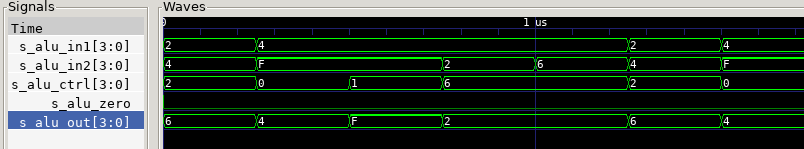
\includegraphics[width=\textwidth]{res/alu.png}

\end{document}
